\documentclass{standalone}

\usepackage{tikz}

\begin{document}

	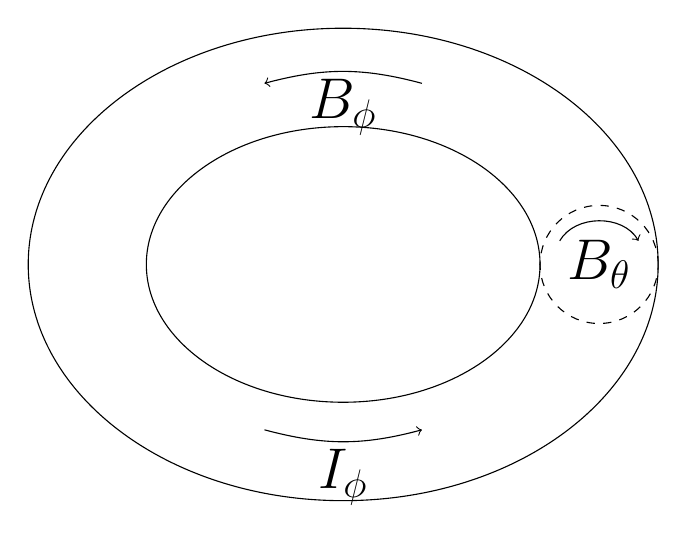
\begin{tikzpicture}
	
	\draw (0,0) ellipse [x radius=4cm, y radius=3cm];

	\draw (0,0) ellipse [x radius=2.5cm, y radius=1.75cm];
	
	\draw[dashed] (3.25,0) circle [radius=0.75cm];
	
	\draw[->]
    (2.75,0.3)
    to [out=60, in=120]
    (3.75,0.3);
    
    \node at (3.25, 0) {\huge \( B_\theta \)};

	\draw[->]
    (1,2.3)
    to [out=165, in=15]
    (-1,2.3);
    
    \node at (0, 2) {\huge \( B_\phi \)};
    
    \draw[->]
    (-1,-2.1)
    to [out=-15, in=195]
    (1,-2.1);
    
    \node at (0, -2.7) {\huge \( I_\phi \)};
	
	\end{tikzpicture}

\end{document}